%!TEX program = xelatex


\documentclass[aspectratio=169]{beamer}
%\documentclass{beamer}

\usepackage{blindtext}

\usepackage{beamerthemeFeecBUT}

\usepackage{xltxtra}
\usepackage[export]{adjustbox}

\usepackage{amssymb}% http://ctan.org/pkg/amssymb
\usepackage{pifont}% http://ctan.org/pkg/pifont
\newcommand{\cmark}{\ding{51}}%
\newcommand{\xmark}{\ding{55}}%
% \usepackage[paperwidth=29cm, paperheight=15cm]{geometry}
% \usepackage[a5paper, landscape]{geometry}

\defaultfontfeatures{Ligatures=TeX}

\def\checkmark{\tikz\fill[scale=0.4](0,.35) -- (.25,0) -- (1,.7) -- (.25,.15) -- cycle;}

\title{Filesystem Consistency Check for Universal Disk Format}
\subtitle{Konference EEICT 2017}
\author{Bc. Vojtěch Vladyka}
\garant{Ing. Petr Petyovský, Ph.D.}
\date{27.dubna 2017}

\begin{document}
	\addtolength{\textwidth}{-20pt}
	\addtolength{\textheight}{-20pt}
  \frame{\titlepage}
   
  \begin{frame}
	\frametitle{Obsah}
	\vspace{40 pt}
	\begin{enumerate}
	  \Large\item Úvod
	  \\ \textcolor{ExecusharesGrey}{\footnotesize\hspace{1em}\large O čem to bude.}	
	  \Large\item Universal Disk Format
	  \\ \textcolor{ExecusharesGrey}{\footnotesize\hspace{1em}\large Co to je UDF?}
	  \Large\item UDF Filesystem Consistency Check
	  \\ \textcolor{ExecusharesGrey}{\footnotesize\hspace{1em}\large A co je to udffsck?}
	  \Large\item Implementace
	  \\ \textcolor{ExecusharesGrey}{\footnotesize\hspace{1em}\large Co je pod kapotou?}
	  \Large\item Závěr
	  \\ \textcolor{ExecusharesGrey}{\footnotesize\hspace{1em}\large Proč vlastně a kudy dál?}
	\end{enumerate}
	\end{frame}

	\section{Úvod}
		\begin{frame}
			\frametitle{Cíl práce}
			\vspace{40 pt}
			\Huge
			\begin{itemize}
				\item\Large Vytvoření nástroje pro detekci a opravu chyb na souborovém systému UDF pro GNU/Linux
				\item\Large Začlenění nástroje do komunity GNU/Linux
			\end{itemize}
		\end{frame}

	\section{Universal Disk Format}
		\begin{frame}
			\frametitle{Co to je?}
            \begin{itemize}
                \Large\item Souborový systém navržený přednostně pro optická média
                \Large\item Náhrada za ISO~9660 (původní souborový systém pro~datová~CD)
                \Large\item První verze vznikla v roce 1995, poslední vydaná (2.60) je~z~roku~2005
                \Large\item Linux umí číst/zapisovat na všechny verze, ale vytvářet jen~do~verze~2.01~(rok 2000)
            \end{itemize}
        \end{frame}
		\begin{frame}
			\frametitle{Struktura}
			\vspace{40 pt}
			\center
            \begin{figure}
			    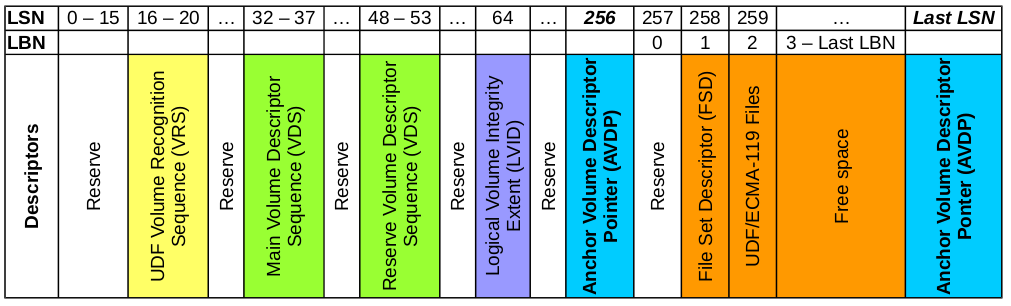
\includegraphics[width=14cm]{UDF-example-schema.png}
                \caption{\Large{Ukázka struktury UDF}}
            \end{figure}
		\end{frame}
	
    \section{UDF Filesystem Consistency Check}
		\begin{frame}
			\frametitle{Co to je?}
			\vspace{40 pt}
            \begin{itemize}
                \Large\item \texttt{fsck} je nástroj pro kontrolu a opravu souborových systémů v unixových operačních systémech
                \Large\item Kontroluje metadata (a žurnály, UDF je nemá) souborových systémů
                \Large\item Pro každý souborový systém je jiný, ale všechny mají stejnou funkci a návratové hodnoty 
            \end{itemize}
            \center
            \LARGE\textbf{\texttt{fsck} neexistuje pro UDF}\\
            \Large{Nebo ano?}
		\end{frame}
        \begin{frame}
            \frametitle{udffsck v září 2016}
			\vspace{40 pt}
			\center
			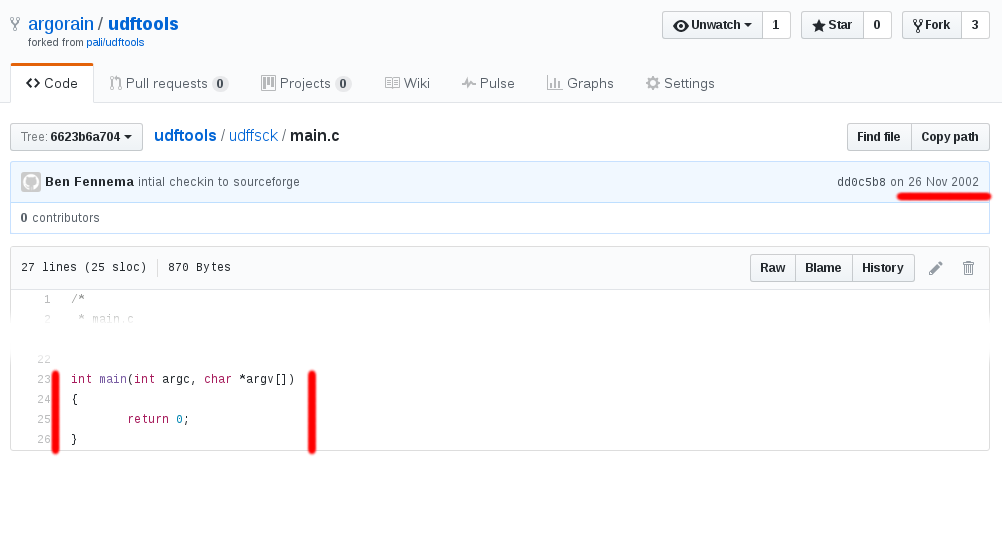
\includegraphics[width=14cm]{github.png}
        \end{frame}
		\begin{frame}
			\frametitle{Detekovatelné a opravitelné chyby}
			\vspace{40 pt}
            \begin{itemize}
                \Large\item Poškození každého deskriptoru (? - záleží na stupni poškození)
                \Large\item Špatné umístění deskriptoru (\cmark)
                \Large\item Nedokončený zápis 
                    \begin{itemize}
                        \large\item Zaalokované místo, ale nezapsaná metadata souboru (\cmark - odstranění nedokončeného souboru)
                        \large\item Zapsaná metadata i data souboru, ale nenavýšený počet souborů (\cmark)
                        \large\item Zapsaná metadata i data souboru, ale neaktualizovaný počet volných bloků (\cmark)
                        \large\item Vše dokončeno, ale neoznačené dokončení práce na systému (\cmark)
                    \end{itemize}
                \Large\item Špatně nastavené časové značky poslední změny (\cmark)
                \Large\item Nenastavené, duplicitní nebo neshodující se Unique ID každého souboru (\cmark)
            \end{itemize}
		\end{frame}
	
    \section{Implementace}
		\begin{frame}
			\frametitle{Balíček udftools}
			\vspace{40 pt}
		    \begin{itemize}
                \Large\item Nástroje pro práci s UDF jsou soustředěny v balíčku udftools
                \Large\item Balíček je vytvořen v jazyce C, build systém je Autotools 
                \Large\item Vývoj začal v roce 2002 Ben Fennema na Sourceforge, poslední změny zanesl v roce 2004
                \Large\item V roce 2014 byl projekt převzat Palim Rohárem který se o něj stará do současnosti
                \Large\item Vývoj \texttt{udffsck} probíhá ve větvi tohoto balíčku a na konci dojde ke sloučení s hlavní větví
            \end{itemize}
        \end{frame}
		\begin{frame}
			\frametitle{Stav implementace} % mmap, flock
			\vspace{40 pt}
		    \begin{itemize}
                \Large\item Implementace standardu UDF až do verze 2.01 (stejná jako zbytek balíčku)  
                \Large\item V současnosti probíhá refactoring kódu pro jeho zveřejnění a testování funkce. Všechny zmíněné metody detekce a korekce jsou implementovány.
                \Large\item Je využíváno mapování souboru (média) do paměti funkcí \texttt{mmap(2)}
                \Large\item Soubor je chráněn proti zápisu po dobu práce funkcí \texttt{flock(2)}
            \end{itemize}
		\end{frame}
        \begin{frame}
            \frametitle{Obsluha nástroje}
            \vspace{40pt}
            \center
            \Large{\texttt{udffsck [-icpvvvh] [-B blocksize] medium}}
            \vspace{20pt}
            \begin{itemize}
                \item\texttt{-B} \textit{Blocksize} - velikost sektoru média v bytech
                \item\texttt{-i} \textit{Interactive} - před každou opravou se dotáže uživatele na schválení
                \item\texttt{-c} \textit{Check only} - pouze zkontroluje médium, nic se nezapíše. Neguje efekt \texttt{-i}
                \item\texttt{-p} \textit{Automatic} - automaticky opraví médium
                \item\texttt{-v} \textit{Verbosity} - zvýšení úrovně výstupu. Bez tohoto nastavení se vypisují pouze chyby, lze navýšit až na \texttt{-vvv} což jsou ladicí výpisy
                \item\texttt{-h} \textit{Help} - nápověda obsahující stručnou pomoc
            \end{itemize}
            %\begin{enumerate}
            %    \item[0] Žádné chyby
            %    \item[1] Nalezené chyby byly opraveny
            %    \item[4] Nalezené chyby zůstaly neopraveny
            %    \item[8] Chyba programu
            %    \item[16] Špatný vstupní parametr
            %    \item[32] Kontrola byla přerušena uživatelem
            %\end{enumerate}
        \end{frame}

        \begin{frame}
            \frametitle{Opravdu pod kapotu}
            \vspace{40pt}
            \center
			
\includegraphics[width=8cm]{github-logo.png}\\
            \LARGE{Pokud opravdu chcete vidět co je uvnitř, doporučuji přímo můj GitHub.}\\
            \vspace{20pt}
            \Large{\url{https://github.com/argorain/udftools}}
        \end{frame}

    \section{Závěr}
		\begin{frame}
			\frametitle{Závěr}
			\vspace{40 pt}
			\Large\textbf{Co se podařilo}
			\begin{itemize}
				\item\Large Vytvořit nástroj, který je schopný kontrolovat a opravovat chyby pro souborový systém UDF v Linuxu 
				\item\Large Pokrytí standardu UDF až po verzi 2.01
				\item\Large Nástroj je funkční na little-endian architekturách
			\end{itemize}
			\Large\textbf{Co je potřeba zlepšit}
			\begin{itemize}
				\item\Large Podpora po poslední verzi 2.60 chybí napříč celým balíčkem, udffsck nevyjímaje
				\item\Large Podporu pro big-endian architektury
			\end{itemize}
			\Large\textbf{Další kroky}
			\begin{itemize}
				\item\Large Začlenění do zdrojového balíčku
			\end{itemize}
		\end{frame}
	    
        \begin{frame}
			\frametitle{Zdroje}
			\vspace{40 pt}
            \begin{itemize}
                \item\emph{Universal Disk Format Specification}. Revision 2.01. Cupertino, California: Optical Storage Technology Association, 2000.
                \item\emph{ECMA-167}. 3rd Edition. Geneva, Switzerland: ECMA, 1997.
                \item\emph{pali/udftools. In: GitHub}\/ [online]. 2016 [cit. 2016-11-21]. Dostupné z: \url{https://github.com/pali/udftools}
            \end{itemize}
		\end{frame}

		\begin{frame}
			\frametitle{Konec}
			\center
			\vspace{40 pt}
			\Huge\textbf{Děkuji za pozornost.}
		\end{frame}

		\begin{frame}
			\frametitle{Konec}
			\center
			\vspace{40 pt}
			\Huge\textbf{Dotazy?}
		\end{frame}
\end{document}
